\begin{figure}[H]
	\centering
	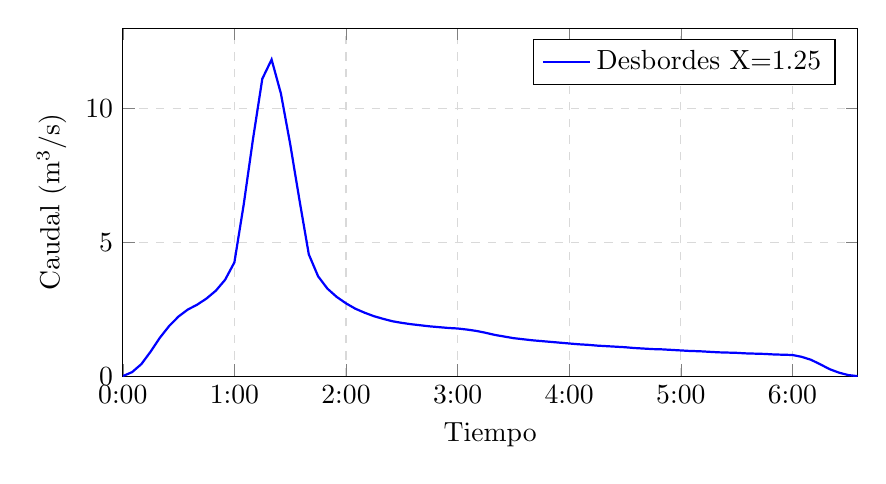
\begin{tikzpicture}
		\begin{axis}[
			width=0.9\textwidth,
			height=6cm,
			xlabel={Tiempo},
			ylabel={Caudal (m$^3$/s)},
			xmin=0,
			xmax=395,
			ymin=0,
			ymax=13,
			grid=major,
			grid style={dashed, gray!30},
			legend pos=north east,
			xtick={0, 60, 120, 180, 240, 300, 360},
			xticklabels={0:00, 1:00, 2:00, 3:00, 4:00, 5:00, 6:00},
			]
		% Desbordes X=1.25
		\addplot [
		blue,
		thick,
		solid,
		] coordinates {
				(0, 0.00) (5, 0.15) (10, 0.45) (15, 0.92) (20, 1.44)
				(25, 1.88) (30, 2.23) (35, 2.49) (40, 2.67) (45, 2.90)
				(50, 3.19) (55, 3.60) (60, 4.25) (65, 6.41) (70, 8.86)
				(75, 11.11) (80, 11.83) (85, 10.56) (90, 8.67) (95, 6.57)
				(100, 4.55) (105, 3.73) (110, 3.27) (115, 2.96) (120, 2.72)
				(125, 2.52) (130, 2.37) (135, 2.24) (140, 2.14) (145, 2.05)
				(150, 1.99) (155, 1.94) (160, 1.90) (165, 1.86) (170, 1.83)
				(175, 1.80) (180, 1.78) (185, 1.74) (190, 1.69) (195, 1.62)
				(200, 1.54) (205, 1.48) (210, 1.42) (215, 1.38) (220, 1.34)
				(225, 1.31) (230, 1.28) (235, 1.25) (240, 1.22) (245, 1.19)
				(250, 1.17) (255, 1.14) (260, 1.12) (265, 1.10) (270, 1.08)
				(275, 1.05) (280, 1.03) (285, 1.01) (290, 1.00) (295, 0.98)
				(300, 0.96) (305, 0.94) (310, 0.93) (315, 0.91) (320, 0.89)
				(325, 0.88) (330, 0.87) (335, 0.85) (340, 0.84) (345, 0.83)
				(350, 0.81) (355, 0.80) (360, 0.79) (365, 0.72) (370, 0.61)
				(375, 0.44) (380, 0.26) (385, 0.13) (390, 0.04) (395, 0.00)
		};
		\addlegendentry{Desbordes X=1.25}

		\end{axis}
	\end{tikzpicture}
	\caption{Hidrograma - Desbordes + GZ $T_r$=25 años ($Q_p$=11.833 m$^3$/s)}
	\label{fig:hydro_desbordes_gz_Tr25_X125}
\end{figure}
